\section{Simulation}

\subsection{Extended Object States and Logical Predicates in \simulator}
\label{as:object_states}
\simulator extends the infrastructure of extended object states and logical predicates from iGibson 2.0~\cite{li2021ig2} to accommodate the diversity and realism of \benchmark.

\subsubsection{Extended object states associated with object category properties}
For computational efficiency purposes, not all extended object states need to be maintained and updated for every object. For example, \texttt{cookable} objects like apples need to keep track of their \texttt{Temperature}, but probably tables don't need to, at least for the purpose of simulating \benchmark activities. Hence, given the object category property annotation from \dataset (see Table~\ref{tab:supp_props}), \simulator selectively keeps track of a subset of the extended states for objects of each category. The mapping from the object category property to the required object states can be found in Table~\ref{table:obj_cat_prop}.
\begin{table}[!htbp]
\begin{center}
{%
\scriptsize
\renewcommand{\arraystretch}{1.2}
\begin{tabular}{ | m{3.5cm} | m{3.7cm} | } 
\hline
\textbf{Object category property} & \textbf{Required extended object states}\\ 
\hline
\texttt{cookable} & \texttt{MaxTemperature}, \texttt{Temperature}\\ 
\hline
\texttt{overcookable} & \texttt{MaxTemperature}, \texttt{Temperature}\\ 
\hline
\texttt{freezable} & \texttt{Temperature}\\ 
\hline
\texttt{flammable} & \texttt{Temperature}\\ 
\hline
\texttt{heatable} & \texttt{Temperature}\\ 
\hline
\texttt{metable} & \texttt{Temperature}\\ 
\hline
\texttt{soakable} & \texttt{SoakedLevel}\\ 
\hline
\texttt{toggleable} & \texttt{ToggledState}\\ 
\hline
\texttt{sliceable} & \texttt{SlicedState}\\ 
\hline
\texttt{breakable} & \texttt{BrokenState}\\ 
\hline
\texttt{heatSource} & \texttt{ToggledState}\\ 
\hline
\texttt{fireSource} & \texttt{ToggledState}\\ 
\hline
\texttt{coldSource} & \texttt{ToggledState}\\ 
\hline
\texttt{waterSource} & \texttt{ToggledState}\\ 
\hline
\end{tabular}
}
\vspace{3pt}
\caption{Extended object states associated with object category properties. Adapted from~\cite{li2021ig2}.}
\label{table:obj_cat_prop}
\end{center}
\end{table}

\subsubsection{Object model properties}
We also need to perform physical and semantic annotation for each object model so that they can be realistically simulated and support the evolution of extended object states. Some of the physical properties can be programmatically generated from the 3D assets, such as \texttt{Shape}, \texttt{KinematicStructure} and  \texttt{StableOrientations}, while others need to be annotated (included in \dataset), such as \texttt{Weight}. \texttt{Type} of an object model, which is also derived from the object category property annotation from \dataset (see Table~\ref{tab:supp_props}), determines how the object will be simulated in \simulator. For example, cloths and fluids will be simulated using underlying particle systems. Also, some of the object category property requires additional semantic annotation for each model of that category, e.g. for \texttt{waterSource} objects, \texttt{WaterSourceLink} is required to indicate the exact location to generate water. An exhaustive list of all the object model properties can be found in Table~\ref{table:obj_model_prob}.
\begin{table}[!htbp]
\begin{center}
%\resizebox{\textwidth}{!}
{%
\scriptsize
\renewcommand{\arraystretch}{1.2}
\begin{tabular}{ | m{2.5cm} | m{2.7cm} | m{7.5cm} | } 
\hline
\textbf{Object model property} & \textbf{Relevant object category property} & \textbf{Description} \\ 
\hline
\texttt{Shape} &  & Model of the 3D shape of each link of the object\\ 
\hline
\texttt{Weight} &  & Weight of the object \\ 
\hline
\texttt{CenterOfMass} &  & Mean position of the matter in the object\\ 
\hline
\texttt{MomentOfInertia} &  & Resistance of the object to change its angular velocity\\ 
\hline
\texttt{KinematicStructure} &  & Structure of links and joints connecting them in the form of URDF (non-articulated objects are composed of one link)\\ 
\hline
\texttt{StableOrientations} &  & A list of stable orientations assuming the object is placed on a flat surface, computed using a 3D geometry library\\ 
\hline
\texttt{HeatSourceLink} & \texttt{heatSource} & Virtual (non-colliding) fixed link that generates heat\\
\hline
\texttt{FireSourceLink} & \texttt{fireSource} & Virtual (non-colliding) fixed link that generates fire\\
\hline
\texttt{CleaningToolLink} & \texttt{cleaningTool} & Fixed link that needs to contact dirt particles for the tool to clean them\\ 
\hline
\texttt{WaterSourceLink} &  \texttt{waterSource} & Virtual (non-colliding) fixed link that generates water\\
\hline
\texttt{WaterSinkLink} &  \texttt{waterSource} & Virtual (non-colliding) fixed link that absorbs water\\ 
\hline
\texttt{TogglingLink} &  \texttt{toggleable} & Virtual (non-colliding) fixed link that changes the toggled state of the object when contacted\\ 
\hline
\texttt{SlicingLink} & \texttt{slicingTool} & Fixed link that changes the sliced state of another object if it contacts it with enough force\\ 
\hline
\texttt{RelevantJoints} & \texttt{openable} & List of joints that are relevant to indicate whether an object is open\\ 
\hline
\texttt{AttachmentKeypoints} & \texttt{assembleable} & List of keypoint locations that will be connected with those of other objects when they are close enough\\ 
\hline
\texttt{ClothKeypoints} & \texttt{foldable}, \texttt{unfoldable} & List of keypoint locations are used to determine if the object is folded (if they are close enough) or unfolded (if they are far enough)\\ 
\hline
\texttt{ContainerVolume} & \texttt{fillable} & Virtual (non-colliding) fixed link that represents the inner volume of a fillable container.\\ 
\hline
\texttt{Type} & \texttt{cloth}, \texttt{deformable}, \texttt{liquid}, \texttt{rope}, \texttt{physicalSubstance}, \texttt{visualSubstance}  & Type of the object, e.g. rigid body, fluid, physical/visual substance, cloth, deformable, which determines how it will be simulated in \simulator \\ 
\hline
\end{tabular}
}
\vspace{3pt}
\caption{Permanent object model properties. Adapted from~\cite{li2021ig2}.}
\label{table:obj_model_prob}
\end{center}
\end{table}

\subsubsection{Object states}
While the object properties mentioned above stay the same during simulation (i.e. an apple is always \texttt{cookable} and a sink always have the same \texttt{WaterSourceLink} defined in its local frame), the object states could change. The underlying physics engine handles the kinematic state changes, such as \texttt{Pose}, \texttt{AABB}, \texttt{JointStates}, \texttt{ParticlePositions} for fluids and cloths, etc. On top of these, \simulator handles the non-kinematic state changes that are essential for logical predicates (described in the next subsection). For example, \simulator update the \texttt{Temperature} of objects at every simulation step by checking if they are near/inside any \texttt{heatSource} or \texttt{coldSource}. An exhaustive list of all the object states can be found in Table~\ref{table:obj_states}.
\begin{table}[!htbp]
\begin{center}
%\resizebox{\textwidth}{!}
{\scriptsize%
\renewcommand{\arraystretch}{1.2}
\begin{tabular}{ | m{4cm} | m{9cm} | } 
\hline
\textbf{Object State} & \textbf{Description and Update Rules} \\ 
\hline
\texttt{Pose} & 6 DoF pose (position and orientation) of the object in world reference frame, updated by the underlying physics engine.\\ 
\hline
\texttt{AABB} & Axis-aligned bounding box (coordinates of two opposite corners) of the object in the world reference frame, updated by the underlying physics engine.\\ 
\hline
\texttt{JointStates} & State of all internal DoFs of the (articulated) object for the structure defined by \texttt{KinematicStructure}, updated by the underlying physics engine.\\ 
\hline
\texttt{ParticlePositions} & Positions of all the underlying particles for cloth and fluid, updated by the underlying physics engine.\\ 
\hline
\texttt{InContactObjs} & List of all objects in physical contact with the object, updated by the underlying physics engine.\\ 
\hline
\texttt{ConnectedObjs} & List of all objects that are connected to the object, either via a fixed joint for rigid bodies or via an attachment for cloth and deformables.\\ 
\hline
\texttt{InSamePositiveVerticalAxisObjs} & List of all objects in the positive vertical axis drawn from the object's center of mass, updated by shooting a ray upwards in the positive z-axis and gather the objects hit by the ray.\\ 
\hline
\texttt{InSameNegativeVerticalAxisObjs} & List of all objects in the negative vertical axis drawn from the object's center of mass, updated by shooting a ray downwards in the negative z-axis and gather the objects hit by the ray.\\ 
\hline
\texttt{InSameHorizontalPlaneObjs} & List of all objects in the horizontal plane drawn from the object's center of mass, updated by shooting a number of ray in the x-y plane and gather the objects hit by the rays.\\ 
\hline
\texttt{Temperature}, $T$ & Object's current temperature in $^\circ$C, updated by detecting if the object is affected by any heat source or heat sink.\\ 
\hline
\texttt{MaxTemperature}, $T_\textit{max}$ & Maximum temperature of the object reached historically during this simulation run, updated by keeping track of all the \texttt{Temperature} in the history.\\ 
\hline
\texttt{SoakedLevel}, $w$ & Amount of liquid absorbed by the object corresponding to the number of liquid particles contacted, updated by detecting if the object is in contact with any liquid particle. This is maintained for every type of \texttt{liquid} separately. \\ 
\hline
\texttt{CoveredLevel}, $c$ & Amount of \texttt{visualSubstance} that covers the object, updated by detecting if the particles of the \texttt{visualSubstance} are in contact with anything that can potentially remove them from the object, e.g. \texttt{cleaningTool}. This is maintained for every type of \texttt{visualSubstance} separately. \\ 
\hline
% \texttt{DustinessLevel}, $d$ & Fraction of the initial amount of dust particles that remain on the object's surface, updated by detecting if the particles are in contact with any \texttt{CleaningTool}.\\ 
% \hline
% \texttt{StainLevel}, $s$ & Fraction of the initial amount of stain particles that remain on the object's surface, updated by detecting if the particles are in contact with any \texttt{Soaked} \texttt{CleaningTool}.\\ 
% \hline
\texttt{ToggledState}, $\textit{TS}$ & Binary state indicating if the object is currently on or off, updated by detecting if the agent is in contact with the \texttt{TogglingLink}.\\ 
\hline
\texttt{SlicedState}, $\textit{SS}$ & Binary state indicating whether the object has been sliced (irreversible), updated by detecting if the object is in contact with any \texttt{SlicingTool} that exerts a force above a certain threshold $F_\mathit{sliced}$. We assume as default force threshold of $F_\mathit{sliced} = \SI{10}{\newton}$, a value that can be configured per object category and model.\\ 
\hline
\texttt{BrokenState}, $\textit{BS}$ & Binary state indicating if the object is broken, updated by detecting if the object has a contact force with any other object above a certain threshold $F_\mathit{broken}$, a value that can be configured per object category and model.\\ 
\hline
\end{tabular}
}
\vspace{3pt}
\caption{Object states maintained by \simulator. Adapted from~\cite{li2021ig2}.}
\label{table:obj_states}
\end{center}
\end{table}

\subsubsection{Logical predicates as checking functions}
For each logical predicate that is relevant for \benchmark activities, we define a checking function that maps a given physical state (kinematic and non-kinematic) into a binary logical state that \bddl operates on. For example, \texttt{OnTopOf} is based on the pose of two objects and their contact information whereas \texttt{Cooked} is based on the \texttt{Temperature}. The details of the checking functions for all the logical predicates can be found in Table~\ref{table:obj_pred_checking}.

\begin{table}[!htbp]
\begin{center}
%\resizebox{\textwidth}{!}
{\scriptsize%
\renewcommand{\arraystretch}{1.2}
\begin{tabular}{ | m{0.20\textwidth} | m{0.7\textwidth} | } 
\hline
\textbf{Predicate} & \textbf{Description} \\ 
\hline
\texttt{InsideOf($o_1$,$o_2$)} & Object $o_1$ is inside of object $o_2$ if we can find two orthogonal axes crossing at $o_1$ center of mass that intersect $o_2$ collision mesh in both directions.\\ 
\hline
\texttt{OnTopOf($o_1$,$o_2$)} & Object $o_1$ is on top of object $o_2$ if $o_2 \in \texttt{InSameNegativeVerticalAxisObjs}(o_1) \land o_2 \not\in \texttt{InSamePositiveVerticalAxisObjs}(o_1) \land \texttt{InContactWith}(o_1, o_2)$, where $\texttt{InSamePositive/NegativeVerticalAxisObjs}(o_1)$ is the list of objects in the same positive/negative vertical axis as $o_1$ and $\texttt{InContactWith}(o_1, o_2)$ is whether the two objects are in physical contact.\\ 
\hline
\texttt{NextTo($o_1$,$o_2$)} & Object $o_1$ is next to object $o_2$ if $o_2 \in \texttt{InSameHorizontalPlaneObjs}(o_1) \land l2(o_1, o_2) < t_\mathit{NextTo}$, where $\texttt{InSameHorizontalPlaneObjs}(o_1)$ is a list of objects in the same horizontal plane as $o_1$, $l2$ is the L2 distance between the closest points of the two objects, and $t_\mathit{NextTo}$ is a distance threshold that is proportional to the average size of the two objects. \\
\hline
\texttt{InContactWith($o_1$,$o_2$)} & Object $o_1$ is in contact with $o_2$ if their surfaces are in contact in at least one point, i.e., $o_2 \in \texttt{InContactObjs}(o_1)$. \\ 
\hline
\texttt{ConnectedWith($o_1$,$o_2$)} & Object $o_1$ is connected with $o_2$ if $o_2 \in \texttt{ConnectedObjs}(o_1)$. \\ 
\hline
\texttt{Under($o_1$,$o_2$)} & Object $o_1$ is under object $o_2$ if $o_2 \in \texttt{InSamePositiveVerticalAxisObjs}(o_1)$ $\land o_2 \not\in \texttt{InSameNegativeVerticalAxisObjs}(o_1)$.\\
\hline
\texttt{OnFloor($o_1$,$o_2$)} & Object $o_1$ is on the room floor $o_2$ if $\texttt{InContactWith}(o_1, o_2)$ and $o_2$ is of \texttt{Room} type. \\ 
\hline
\texttt{Open(o)} & Any joints (internal articulated degrees of freedom) of object $o$ are open. Only joints that are relevant to consider an object \texttt{Open} are used in the predicate computation, e.g. the door of a microwave but not the buttons and controls. To select the relevant joints, object models of categories that can be \texttt{Open} undergo an additional annotation that produces a \texttt{RelevantJoints} list. A joint is considered open if its joint state $q$ is 5\% over the lower limit, i.e. $q > 0.05(q_\mathit{UpperLimit} - q_\mathit{LowerLimit}) + q_\mathit{LowerLimit}$. \\
\hline
\texttt{Cooked(o)} & The temperature of object $o$ was over the cooked threshold, $T_\mathit{cooked}$, and under the burnt threshold, $T_\mathit{burnt}$, at least once in the history of the simulation episode, i.e., $T_\mathit{cooked} \leq T_o^\mathit{max} < T_\mathit{burnt}$. We annotate the cooked temperature $T_\mathit{cooked}$ for each object category that can be \texttt{Cooked}.\\
\hline
\texttt{Burnt(o)} & The temperature of object $o$ was over the burnt threshold, $T_\mathit{burnt}$, at least once in the history of the simulation episode, i.e., $T_o^\mathit{max} \geq T_\mathit{burnt}$. We annotate the burnt temperature $T_\mathit{burnt}$ for each object category that can be \texttt{Burnt}.\\
\hline
\texttt{OnFire(o)} & The temperature of object $o$ is above the on-fire threshold, $T_\mathit{onfire}$, i.e., $T_o \leq T_\mathit{onfire}$. We assume as default on-fire temperature $T_\mathit{onfire}=300^\circ C$, a value that can be adapted per object category and model.\\
\hline
\texttt{Frozen(o)} & The temperature of object $o$ is under the freezing threshold, $T_\mathit{frozen}$, i.e., $T_o \leq T_\mathit{frozen}$. We assume as default freezing temperature $T_\mathit{frozen}=0^\circ C$, a value that can be adapted per object category and model.\\
\hline
\texttt{Heated(o)} & The temperature of object $o$ is above the heated threshold, $T_\mathit{heated}$, i.e., $T_o \leq T_\mathit{heated}$. We assume as default heated temperature $T_\mathit{heated}=75^\circ C$, a value that can be adapted per object category and model.\\
\hline
\texttt{Boiled(l)} & The temperature of liquid $l$ is above the boiling point, $T_\mathit{boiled}$, i.e., $T_o \leq T_\mathit{boiled}$. We assume as default boiling point $T_\mathit{boiling}=100^\circ C$, a value that can be adapted per object category and model.\\
\hline
\texttt{Soaked(o, l)} & The soaked level $w$ of the liquid $l$ for the object $o$ is over a threshold, $w_\mathit{soaked}$, i.e., $w \geq w_\mathit{soaked}$. The default value for the threshold is $w_\mathit{soaked}=50$, (the object is soaked if it absorbs more than $50$ liquid particles), a value that can be adapted per object category and model and per liquid type.\\
\hline

\texttt{Filled(o, l)} & Object $o$ is filled by liquid $l$ if the number of particles of $l$ that is inside the \texttt{ContainerVolume} of $o$ is above a certain threshold percentage of the total volume. The default value for the threshold is $w_\mathit{filled}=0.5$. \\
\hline
\texttt{Covered(o, s)} & For \texttt{visualSubstance} $s$, check if the covered level $c$ of $s$ for the object $o$ is over a threshold, $c_\mathit{covered}$, i.e., $c \geq c_\mathit{covered}$; for \texttt{physicalSubstance} $s$, check if the number of particles of $s$ that are in contact with the object $o$ is over the same threshold. The default value for the threshold is $c_\mathit{covered}=50$ (50 substance particles), a value that can be adapted per object category and model, and per substance.\\
\hline
% \texttt{Dusty(o)} &  The  dustiness level $d$ of the object $o$ is over a threshold, $d_\mathit{dusty}$, i.e., $d > d_\mathit{dusty}$. The default value for the threshold is $d_\mathit{dusty}=0.5$, (half of the dust particles have been cleaned), a value that can be adapted per object category and model.\\
% \hline
% \texttt{Stained(o)} &   The  stain level $s$ of the object $o$ is over a threshold, $s_\mathit{stained}$, i.e., $s > s_\mathit{stained}$. The default value for the threshold is $s_\mathit{stained}=0.5$, (half of the stain particles have been cleaned), a value that can be adapted per object category and model.\\
% \hline
\texttt{ToggledOn(o)} & Object $o$ is toggled on or off. It is a direct query of the object's extended state $\mathit{TS}$, the toggled state.\\ 
\hline
\texttt{Sliced(o)} & Object $o$ is sliced or not. It is a direct access of the object's extended state $\mathit{SS}$, the sliced state.\\
\hline
\texttt{Broken(o)} & Object $o$ is broken or not. It is a direct access of the object's extended state $\mathit{BS}$, the broken state.\\
\hline
\texttt{Folded(o)} & Object $o$ is folded if its corresponding \texttt{ClothKeypoints} are sufficiently close to each other.\\
\hline
\texttt{Unfolded(o)} & Object $o$ is unfolded if its corresponding \texttt{ClothKeypoints} are sufficiently far from each other.\\
\hline
\texttt{Assembled(o)} & Object $o$ is assembled if all of its parts have been correctly connected: every pair of parts $p_i$ and $p_j$ are connected (or not) with each other (i.e. $\texttt{IsConnected}(p_i, p_j)$) in a specific way defined by each object model.\\
\hline
\texttt{Hung($o_1$,$o_2$)} & Object $o_1$ is hung onto object $o_2$ if they are connected, $\texttt{IsConnected}(o_1, o_2)$.\\
\hline
\texttt{Blended($o_1$ ... $o_n$)} & Objects $o_1$ to $o_n$ are blended if they are in contact with each other, i.e. $\texttt{InContactWith}(o_i, o_j)$ for all pairs.\\
\hline
\texttt{InFoVOfAgent(o)} & Object $o$ is in the field of view of the agent, i.e., at least one pixel of the image acquired by the agent's onboard sensors corresponds to the surface of $o$.\\
\hline
\texttt{InHandOfAgent(o)} & Object $o$ is grasped by the agent's hands (i.e. assistive grasping is activated on that object).\\
\hline
\texttt{InReachOfAgent(o)} & Object $o$ is within $d_\mathit{reach}=2$ meters away from the agent.\\
\hline
\texttt{InSameRoomAsAgent(o)} & Object $o$ is located in the same room as the agent.\\
\hline
\end{tabular}
}
\vspace{3pt}
\caption{\textbf{Logical Predicates:} Description of the checking functions. Adapted from~\cite{li2021ig2}.}
\label{table:obj_pred_checking}
\end{center}
\end{table}

\subsubsection{Logical predicates as sampling functions}
For each logical predicate that is relevant for \benchmark activities, we also define a generative function that samples a valid physical state given a binary logical state. This functionality is essential for infinite activity initialization. For example, if the initial conditions of the activity require a plate to be \texttt{OnTopOf} a dining table, there are an infinite number of exact poses of the plate that can satisfy this condition. Our generative functions will find a valid solution and physically put the plate on top of the table. Other examples include setting the \texttt{Temperature} of an object to make it \texttt{Frozen} or the joint configuration of an object to make it \texttt{Open}. The details of the sampling functions for all the logical predicates can be found in Table~\ref{table:obj_pred_checking}.

\begin{table}[!t]
\begin{center}
%\resizebox{\textwidth}{!}
{\scriptsize%
\renewcommand{\arraystretch}{1.2}
\begin{tabular}{ | m{0.20\textwidth} | m{0.7\textwidth} | } 
\hline
\textbf{Predicate} & \textbf{Sampling Mechanism} \\ 
\hline
\texttt{InsideOf($o_1$,$o_2$)} & Only \texttt{InsideOf($o_1$,$o_2$) = True} can be sampled. $o_1$ is randomly sampled within $o_2$ using a ray-casting mechanism adopted from~\cite{srivastava2021behavior}. $o_1$ is guaranteed to be supported fully by a surface and free of collisions with any other object except $o_2$.\\ 
\hline
\texttt{OnTopOf($o_1$,$o_2$)} & Only \texttt{OnTopOf($o_1$,$o_2$) = True} can be sampled. $o_1$ is randomly sampled on top of $o_2$ using a ray-casting mechanism adopted from~\cite{srivastava2021behavior}. $o_1$ is guaranteed to be supported fully by a surface and free of collisions with any other object except $o_2$.\\ 
\hline
% \texttt{NextTo($o_1$,$o_2$)} & Not supported at the moment. \\
% \hline
% \texttt{InContactWith($o_1$,$o_2$)} & Not supported at the moment. \\ 
% \hline
\texttt{ConnectedWith($o_1$,$o_2$)} & Create a rigid joint between the two objects if they are both rigid bodies, or an attachment between them otherwise.\\ 
\hline
\texttt{Under($o_1$,$o_2$)} & Only \texttt{Under($o_1$,$o_2$) = True} can be sampled. $o_1$ is randomly sampled on top of the floor region beneath $o_2$ using a ray-casting mechanism adopted from~\cite{srivastava2021behavior}. $o_1$ is guaranteed to be supported fully by a surface and free of collisions with any other object except the floor.\\
\hline
\texttt{OnFloor($o_1$,$o_2$)} & Only \texttt{OnFloor($o_1$,$o_2$) = True} can be sampled. $o_1$ is randomly sampled on top of $o_2$, which is the floor of a certain room, using the scene's room segmentation mask. $o_1$ is guaranteed to be supported fully by a surface and free of collisions with any other object except $o_2$.\\ 
\hline
\texttt{Open(o)} & To sample an object $o$ with the predicate \texttt{Open(o) = True}, a subset of the object's relevant joints (using the \texttt{RelevantJoints} model property) are selected, and each selected joint is moved to a uniformly random position between the openness threshold and the joint's upper limit. To sample an object $o$ with the predicate \texttt{Open(o) = False}, all of the object's relevant joints (using the \texttt{RelevantJoints} model property) are moved to a uniformly random position between the joint's lower limit and the openness threshold.\\
\hline
\texttt{Cooked(o)} & To sample an object $o$ with the predicate \texttt{Cooked(o) = True}, the object's \texttt{MaxTemperature} is updated to $\max(T_o^\mathit{max}, T_\mathit{cooked})$. Similarly, to sample an object $o$ with the predicate \texttt{Cooked(o) = False}, the object's \texttt{MaxTemperature} is updated to $\min(T_o^\mathit{max}, T_\mathit{cooked} - 1)$. \\
\hline
\texttt{Burnt(o)} & To sample an object $o$ with the predicate \texttt{Burnt(o) = True}, the object's \texttt{MaxTemperature} is updated to $\max(T_o^\mathit{max}, T_\mathit{burnt})$. Similarly, to sample an object $o$ with the predicate \texttt{Cooked(o) = False}, the object's \texttt{MaxTemperature} is updated to $\min(T_o^\mathit{max}, T_\mathit{burnt} - 1)$.\\
\hline
\texttt{OnFire(o)} & To sample an object $o$ with the predicate \texttt{OnFire(o) = True}, the object's \texttt{Temperature} is updated to a uniformly random temperature between $T_\mathit{onfire} + 10$ and $T_\mathit{onfire} + 50$. To sample an object $o$ with the predicate \texttt{OnFire(o) = False}, the object's \texttt{Temperature} is updated to $T_\mathit{onfire} - 1$. \\
\hline
\texttt{Frozen(o)} & To sample an object $o$ with the predicate \texttt{Frozen(o) = True}, the object's \texttt{Temperature} is updated to a uniformly random temperature between $T_\mathit{frozen} - 10$ and $T_\mathit{frozen} - 50$. To sample an object $o$ with the predicate \texttt{Frozen(o) = False}, the object's \texttt{Temperature} is updated to $T_\mathit{frozen} + 1$. \\
\hline
\texttt{Heated(o)} & To sample an object $o$ with the predicate \texttt{Heated(o) = True}, the object's \texttt{Temperature} is updated to a uniformly random temperature between $T_\mathit{heated} + 10$ and $T_\mathit{heated} + 50$. To sample an object $o$ with the predicate \texttt{Heated(o) = False}, the object's \texttt{Temperature} is updated to $T_\mathit{heated} - 1$. \\
\hline
\texttt{Boiled(l)} & To sample a liquid type $l$ with the predicate \texttt{Boiled(l) = True}, the \texttt{Temperature} of all particles of $l$ is updated to a uniformly random temperature between $T_\mathit{boiled} + 10$ and $T_\mathit{boiled} + 50$. To sample a liquid type $l$ with the predicate \texttt{Boiled(o) = False}, the \texttt{Temperature} of all particles of $l$ is updated to $T_\mathit{boiled} - 1$. \\
\hline
\texttt{Soaked(o, l)} & To sample an object $o$ and a liquid type $l$ with the predicate \texttt{Soaked(o, l) = True}, the object's \texttt{SoakedLevel} $w$ for $l$ is updated to match the \texttt{Soaked} threshold of $w_\mathit{soaked}$. To sample an object $o$ and a liquid type $l$ with the predicate \texttt{Soaked(o, l) = False}, the object's \texttt{SoakedLevel} $w$ is updated to 0.\\
\hline
\texttt{Filled(o, l)} & To sample an object $o$ and a liquid type $l$ with the predicate \texttt{Filled(o, l) = True}, an appropriate number of particles of $l$ are sampled inside the \texttt{ContainerVolume} of $o$ so that they fill up enough of its volume ($\geq w_\mathit{filled}=0.5$). To sample an object $o$ and a liquid type $l$ with the predicate \texttt{Filled(o, l) = False}, all particles of $l$ that are inside the \texttt{ContainerVolume} of $o$ (if any) are removed.\\
\hline
\texttt{Covered(o, s)} & To sample an object $o$ and a substance $s$ with \texttt{Covered(o, s) = True}, a fixed number of particles of $s$ are randomly placed on the surface of $o$ using a ray-casting mechanism adopted from~\cite{srivastava2021behavior}. To sample an object $o$  and a \texttt{visualSubstance} $s$ with \texttt{Covered(o, s) = False}, all particles of $s$ is removed from $o$ and the corresponding \texttt{CoveredLevel} is set to 0.\\
\hline
% \texttt{Dusty(o)} & To sample an object with \texttt{Dusty(o) = True}, a fixed number (currently 20) of dust particles are randomly placed on the surface of $o$ using the mechanism described in Pose Sampling Algorithm in Sec.~\ref{ss:kinematicsampling}. To sample an object with \texttt{Dusty(o) = False}, all dust particles on the object are removed.\\
% \hline
% \texttt{Stained(o)} & To sample an object with \texttt{Stained(o) = True}, a fixed number (currently 20) of stain particles are randomly placed on the surface of $o$ using the mechanism described in Pose Sampling ALgorithm in Sec.~\ref{ss:kinematicsampling}. To sample an object with \texttt{Stained(o) = False}, all stain particles on the object are removed.\\
% \hline
\texttt{ToggledOn(o)} & The \texttt{ToggledState} of the object is updated to match the required predicate value. \\ 
\hline
\texttt{Sliced(o)} & The \texttt{SlicedState} of the object is updated to match the required predicate value. Also, the whole object are replaced with the two halves, that will be placed at the same location and inherit the extended states from the whole object (e.g. \texttt{Temperature}).\\
\hline
\texttt{Broken(o)} & The \texttt{BrokenState} of the object is updated to match the required predicate value. Also, the whole object is broken down into pieces, that will be placed at the same location.\\
\hline
% \texttt{Folded(o)} & Not supported at the moment.\\
% \hline
% \texttt{Unfolded(o)} & Not supported at the moment.\\
% \hline
% \texttt{Assembled(o)} & Not supported at the moment.\\
% \hline
% \texttt{Hung($o_1$, $o_2$)} & Not supported at the moment.\\
% \hline
% \texttt{Blended($o_1$ ... $o_n$)} & Not supported at the moment. \\
% \hline
% \texttt{InFoVOfAgent(o)} & Not supported at the moment. \\
% \hline
% \texttt{InHandOfAgent(o)} & Not supported at the moment.\\
% \hline
% \texttt{InReachOfAgent(o)} & Not supported at the moment.\\
% \hline
% \texttt{InSameRoomAsAgent(o)} & Not supported at the moment.\\
% \hline
\end{tabular}
}
\vspace{3pt}
\caption{\textbf{Logical Predicates:} Description of the sampling functions. Adapted from~\cite{li2021ig2}.}
\label{table:obj_pred_sampling}
\end{center}
\end{table}

% \begin{figure}[t]
%     \centering
%     \includegraphics[width=0.95\textwidth]{figures/omnigibson/Omni_Transition_Map.png}
%     \caption{[In appendix] Transition maps visualization: two cooking recipes and two cleaning formulas. This shows the realism of B1K activity definition. }
%     \label{fig:activity_transition}
% \end{figure}

\subsection{AMT Visual Realism Study}
\label{amt_study_appx}

We conducted an Amazon Mechanical Turk (AMT) study to evaluate \simulator's relative visual realism compared to multiple other simulation environments. We selected 50 representative $1280 \times 720$ images from \simulator, AI2-Thor, ThreeDWorld, Habitat 2.0, and iGibson 2.0, and shuffled them randomly into 50 groups of 5 images, where each group contained a unique image from each simulation environment. For each group, participants were asked to rank the images in terms of visual realism, assigning the most realistic images of the group $1$, and subsequent images $2, ..., 5$. Image shuffling was randomized between participants. When presenting our results, we invert the aggregated mean and standard deviation across 60 participants, such that a score of a $5$ would represent the most visually realistic images.

%Below, we include all 50 images used from each simulation platform.
Our criteria for selecting the images are the following: (a) we only included photos taken from \textit{fully interactive} scenes for a fair comparison, and (b) rendering must come from within the simulation environment, without customized tuning (i.e. new users can expect this visual quality off-the-shelf with minimal adjustment).

\begin{figure}[t]
\centering
\captionsetup[subfigure]{aboveskip=1pt,belowskip=1pt}
\begin{subfigure}[t]{0.304\textwidth}{%
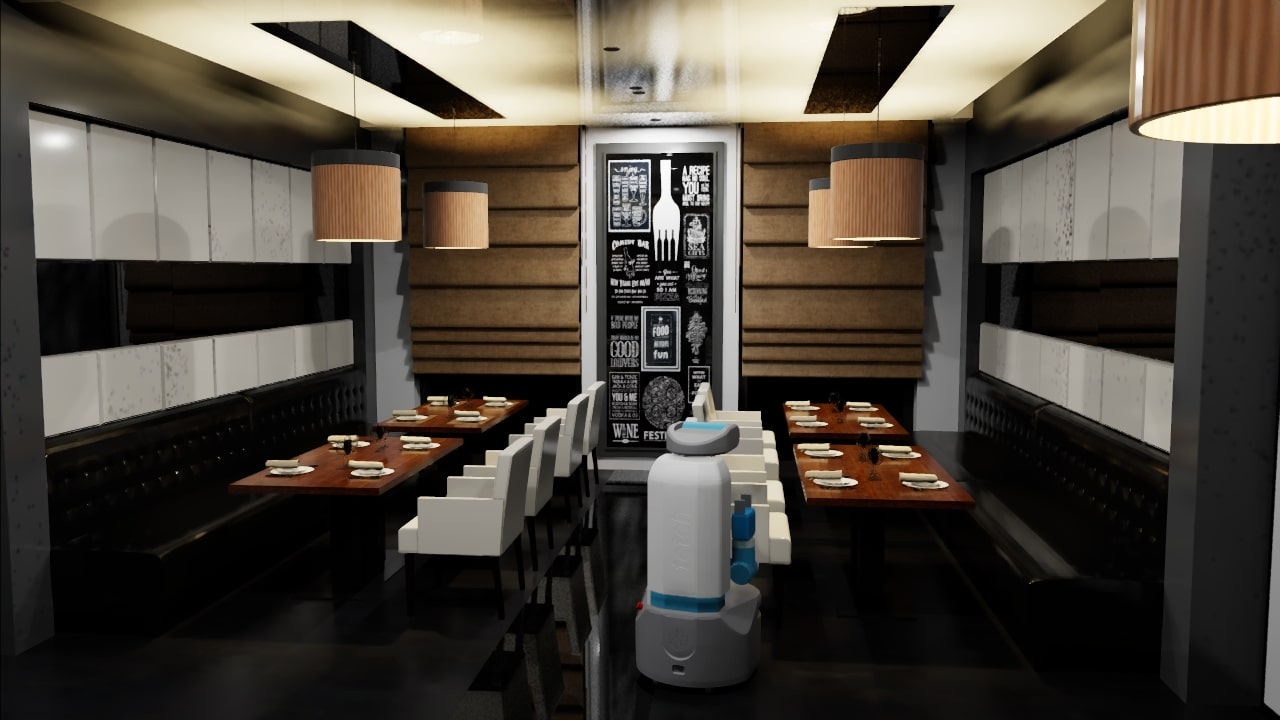
\includegraphics[width=\textwidth]{figures/omnigibson/robot_images/third_pov.jpg}}%
\caption*{\scriptsize3rd Person View}%
\end{subfigure}%
\hfill%
%\subfloat[][\scriptsize RGB]
\begin{subfigure}[t]{0.17\textwidth}{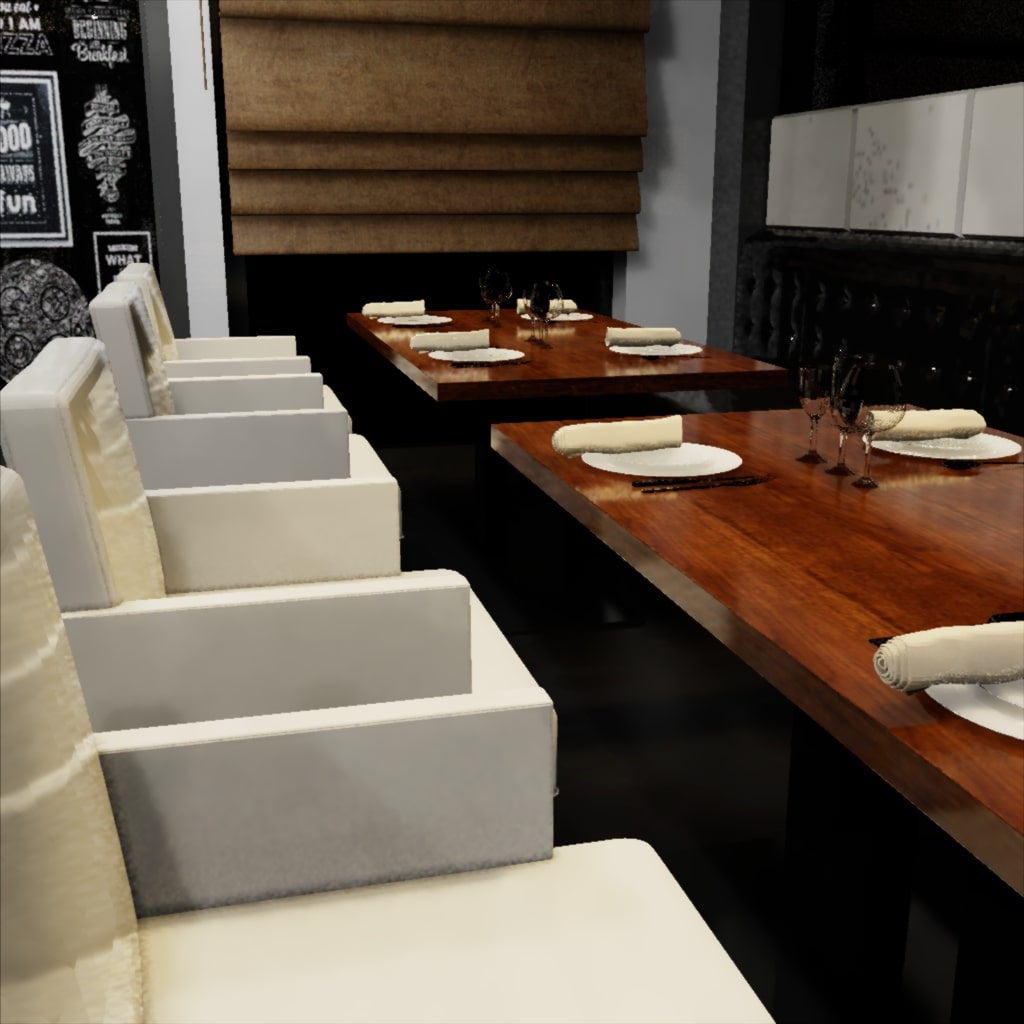
\includegraphics[width=\textwidth]{figures/omnigibson/robot_images/rgb.jpg}}%
\caption*{\scriptsize RGB}%
\end{subfigure}%
\hfill%
%\subfloat[][\scriptsize Depth]
\begin{subfigure}[t]{0.17\textwidth}{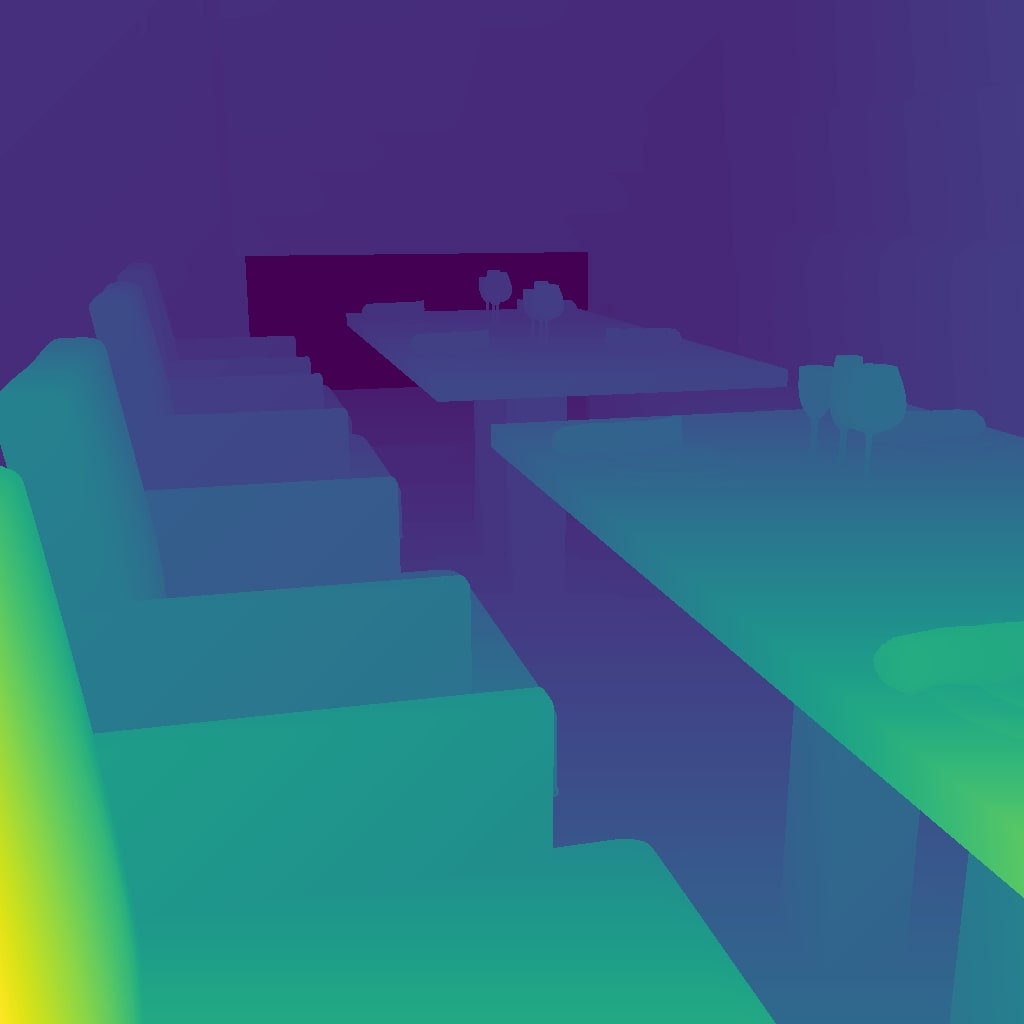
\includegraphics[width=\textwidth]{figures/omnigibson/robot_images/depth.jpg}}%
\caption*{\scriptsize Depth}%
\end{subfigure}%
\hfill%
%\subfloat[][\scriptsize Normals]
\begin{subfigure}[t]{0.17\textwidth}{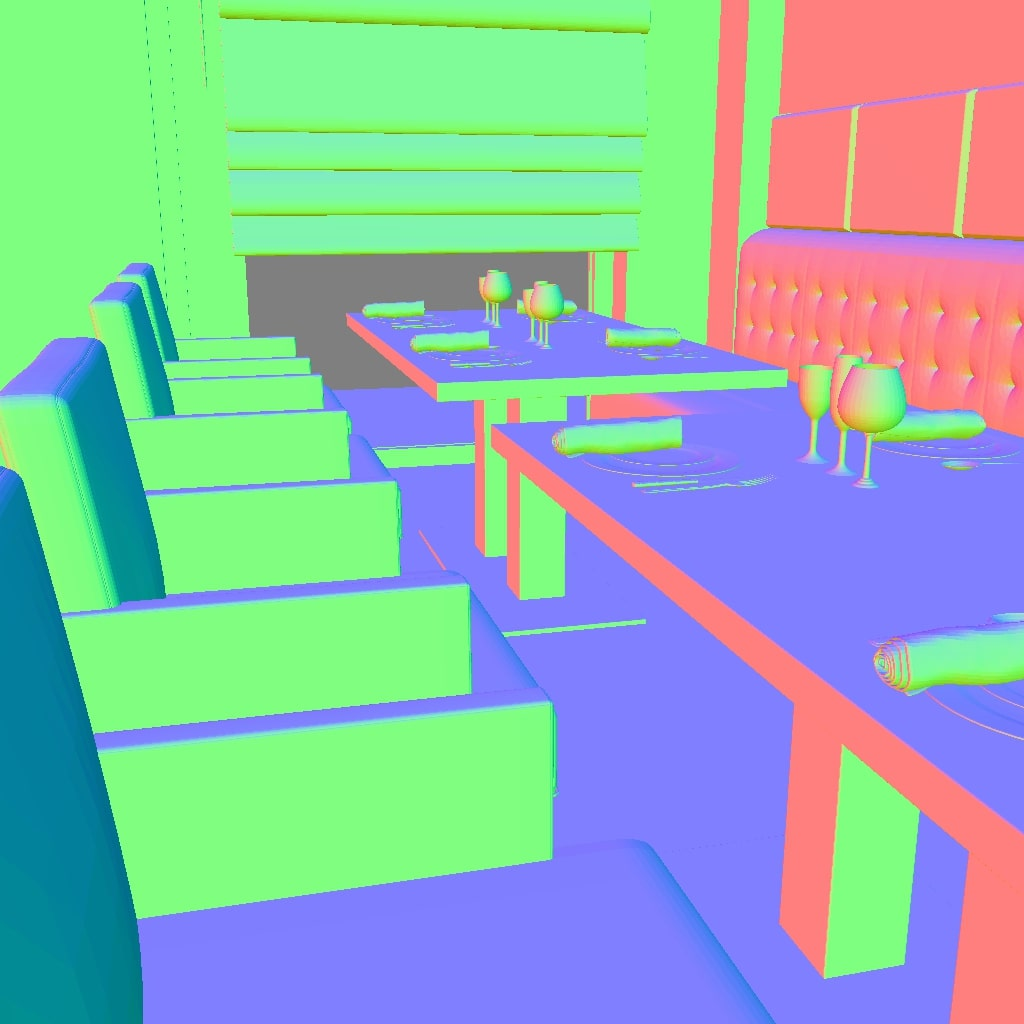
\includegraphics[width=\textwidth]{figures/omnigibson/robot_images/normal.jpg}}%
\caption*{\scriptsize Normals}%
\end{subfigure}%
\hfill%
% \subfloat[][\scriptsize Inst. Segm.]
\begin{subfigure}[t]{0.17\textwidth}{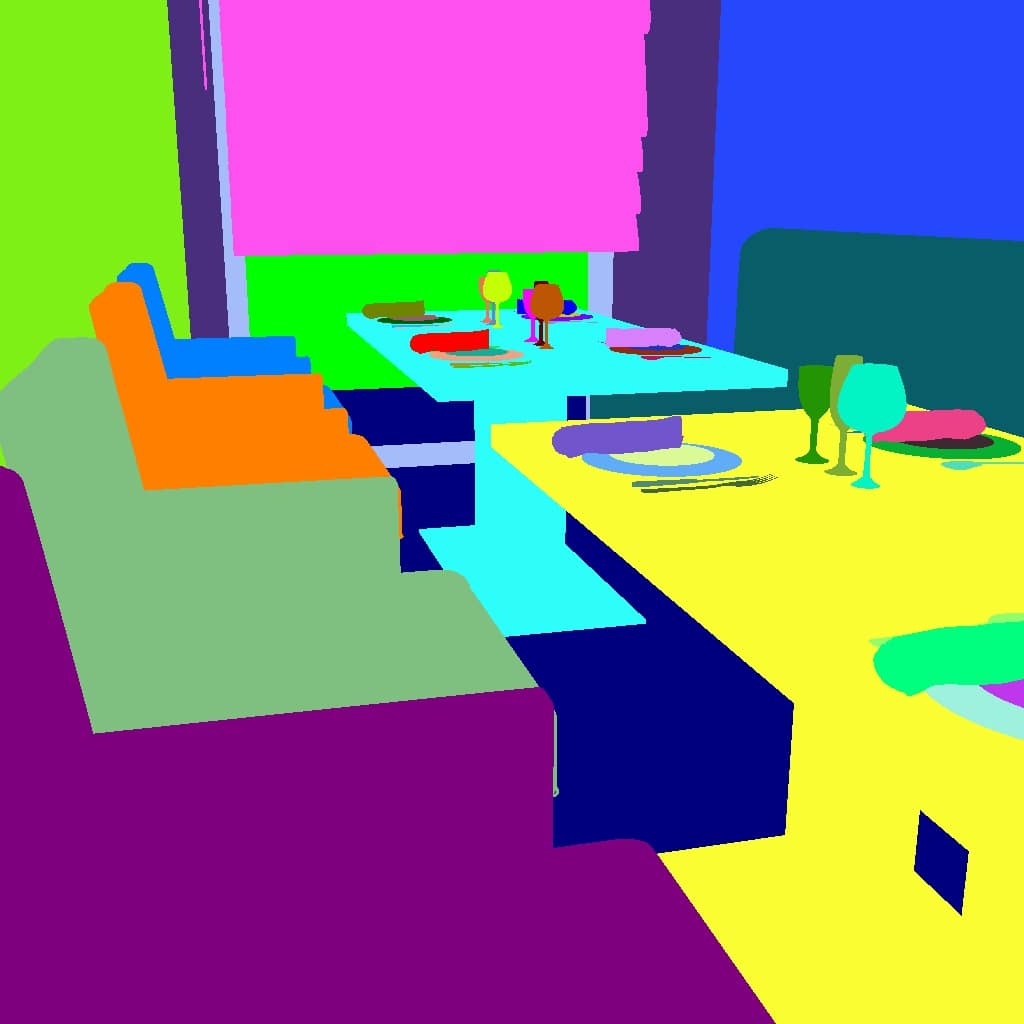
\includegraphics[width=\textwidth]{figures/omnigibson/robot_images/seg_instance.jpg}}%
\caption*{\scriptsize Inst. Segm.}%
\end{subfigure}%
\captionsetup[figure]{font=small,skip=-2pt}%
\caption{\textbf{Visual modalities provided by \simulator.} The robot observes the scene (left, 3rd person view) and obtains visual observations from its onboard sensors including RGB images, depth, normals, and instance segmentation. Rendered RGB images are highly realistic, and, combined with the diverse set of visual observations, can be used to train visual policies.}
\label{fig:sim_modalities}
\end{figure}

% 
\begin{figure}[t]
\captionsetup[subfloat]{labelformat=empty}
\captionsetup[subfloat]{justification=centering}
\centering

\subfloat[\simulator]{}
\hfill
\subfloat[][AI2-Thor]{}
\hfill
\subfloat[][ThreeDWorld]{}
\hfill
\subfloat[][Habitat 2.0]{}
\hfill
\subfloat[][iGibson 2.0]{}

\subfloat[][]{\includegraphics[width=.199\textwidth]{figures/omnigibson/amt_study/og/1.jpg}}
\hfill
\subfloat[][]{\includegraphics[width=.199\textwidth]{figures/omnigibson/amt_study/ai2/1.jpg}}
\hfill
\subfloat[][]{\includegraphics[width=.199\textwidth]{figures/omnigibson/amt_study/tdw/1.jpg}}
\hfill
\subfloat[][]{\includegraphics[width=.199\textwidth]{figures/omnigibson/amt_study/habitat/1.jpg}}
\hfill
\subfloat[][]{\includegraphics[width=.199\textwidth]{figures/omnigibson/amt_study/ig2/1.jpg}}

\vspace{-6pt}

\subfloat[][]{\includegraphics[width=.199\textwidth]{figures/omnigibson/amt_study/og/2.jpg}}
\hfill
\subfloat[][]{\includegraphics[width=.199\textwidth]{figures/omnigibson/amt_study/ai2/2.jpg}}
\hfill
\subfloat[][]{\includegraphics[width=.199\textwidth]{figures/omnigibson/amt_study/tdw/2.jpg}}
\hfill
\subfloat[][]{\includegraphics[width=.199\textwidth]{figures/omnigibson/amt_study/habitat/2.jpg}}
\hfill
\subfloat[][]{\includegraphics[width=.199\textwidth]{figures/omnigibson/amt_study/ig2/2.jpg}}

\vspace{-6pt}

\subfloat[][]{\includegraphics[width=.199\textwidth]{figures/omnigibson/amt_study/og/3.jpg}}
\hfill
\subfloat[][]{\includegraphics[width=.199\textwidth]{figures/omnigibson/amt_study/ai2/3.jpg}}
\hfill
\subfloat[][]{\includegraphics[width=.199\textwidth]{figures/omnigibson/amt_study/tdw/3.jpg}}
\hfill
\subfloat[][]{\includegraphics[width=.199\textwidth]{figures/omnigibson/amt_study/habitat/3.jpg}}
\hfill
\subfloat[][]{\includegraphics[width=.199\textwidth]{figures/omnigibson/amt_study/ig2/3.jpg}}

\vspace{-6pt}

\subfloat[][]{\includegraphics[width=.199\textwidth]{figures/omnigibson/amt_study/og/4.jpg}}
\hfill
\subfloat[][]{\includegraphics[width=.199\textwidth]{figures/omnigibson/amt_study/ai2/4.jpg}}
\hfill
\subfloat[][]{\includegraphics[width=.199\textwidth]{figures/omnigibson/amt_study/tdw/4.jpg}}
\hfill
\subfloat[][]{\includegraphics[width=.199\textwidth]{figures/omnigibson/amt_study/habitat/4.jpg}}
\hfill
\subfloat[][]{\includegraphics[width=.199\textwidth]{figures/omnigibson/amt_study/ig2/4.jpg}}

\vspace{-6pt}

\subfloat[][]{\includegraphics[width=.199\textwidth]{figures/omnigibson/amt_study/og/5.jpg}}
\hfill
\subfloat[][]{\includegraphics[width=.199\textwidth]{figures/omnigibson/amt_study/ai2/5.jpg}}
\hfill
\subfloat[][]{\includegraphics[width=.199\textwidth]{figures/omnigibson/amt_study/tdw/5.jpg}}
\hfill
\subfloat[][]{\includegraphics[width=.199\textwidth]{figures/omnigibson/amt_study/habitat/5.jpg}}
\hfill
\subfloat[][]{\includegraphics[width=.199\textwidth]{figures/omnigibson/amt_study/ig2/5.jpg}}

\vspace{-6pt}

\subfloat[][]{\includegraphics[width=.199\textwidth]{figures/omnigibson/amt_study/og/6.jpg}}
\hfill
\subfloat[][]{\includegraphics[width=.199\textwidth]{figures/omnigibson/amt_study/ai2/6.jpg}}
\hfill
\subfloat[][]{\includegraphics[width=.199\textwidth]{figures/omnigibson/amt_study/tdw/6.jpg}}
\hfill
\subfloat[][]{\includegraphics[width=.199\textwidth]{figures/omnigibson/amt_study/habitat/6.jpg}}
\hfill
\subfloat[][]{\includegraphics[width=.199\textwidth]{figures/omnigibson/amt_study/ig2/6.jpg}}

\vspace{-6pt}

\subfloat[][]{\includegraphics[width=.199\textwidth]{figures/omnigibson/amt_study/og/7.jpg}}
\hfill
\subfloat[][]{\includegraphics[width=.199\textwidth]{figures/omnigibson/amt_study/ai2/7.jpg}}
\hfill
\subfloat[][]{\includegraphics[width=.199\textwidth]{figures/omnigibson/amt_study/tdw/7.jpg}}
\hfill
\subfloat[][]{\includegraphics[width=.199\textwidth]{figures/omnigibson/amt_study/habitat/7.jpg}}
\hfill
\subfloat[][]{\includegraphics[width=.199\textwidth]{figures/omnigibson/amt_study/ig2/7.jpg}}

\vspace{-6pt}

\subfloat[][]{\includegraphics[width=.199\textwidth]{figures/omnigibson/amt_study/og/8.jpg}}
\hfill
\subfloat[][]{\includegraphics[width=.199\textwidth]{figures/omnigibson/amt_study/ai2/8.jpg}}
\hfill
\subfloat[][]{\includegraphics[width=.199\textwidth]{figures/omnigibson/amt_study/tdw/8.jpg}}
\hfill
\subfloat[][]{\includegraphics[width=.199\textwidth]{figures/omnigibson/amt_study/habitat/8.jpg}}
\hfill
\subfloat[][]{\includegraphics[width=.199\textwidth]{figures/omnigibson/amt_study/ig2/8.jpg}}

\vspace{-6pt}

\subfloat[][]{\includegraphics[width=.199\textwidth]{figures/omnigibson/amt_study/og/9.jpg}}
\hfill
\subfloat[][]{\includegraphics[width=.199\textwidth]{figures/omnigibson/amt_study/ai2/9.jpg}}
\hfill
\subfloat[][]{\includegraphics[width=.199\textwidth]{figures/omnigibson/amt_study/tdw/9.jpg}}
\hfill
\subfloat[][]{\includegraphics[width=.199\textwidth]{figures/omnigibson/amt_study/habitat/9.jpg}}
\hfill
\subfloat[][]{\includegraphics[width=.199\textwidth]{figures/omnigibson/amt_study/ig2/9.jpg}}

\vspace{-6pt}

\subfloat[][]{\includegraphics[width=.199\textwidth]{figures/omnigibson/amt_study/og/10.jpg}}
\hfill
\subfloat[][]{\includegraphics[width=.199\textwidth]{figures/omnigibson/amt_study/ai2/10.jpg}}
\hfill
\subfloat[][]{\includegraphics[width=.199\textwidth]{figures/omnigibson/amt_study/tdw/10.jpg}}
\hfill
\subfloat[][]{\includegraphics[width=.199\textwidth]{figures/omnigibson/amt_study/habitat/10.jpg}}
\hfill
\subfloat[][]{\includegraphics[width=.199\textwidth]{figures/omnigibson/amt_study/ig2/10.jpg}}

\vspace{-6pt}

\subfloat[][]{\includegraphics[width=.199\textwidth]{figures/omnigibson/amt_study/og/11.jpg}}
\hfill
\subfloat[][]{\includegraphics[width=.199\textwidth]{figures/omnigibson/amt_study/ai2/11.jpg}}
\hfill
\subfloat[][]{\includegraphics[width=.199\textwidth]{figures/omnigibson/amt_study/tdw/11.jpg}}
\hfill
\subfloat[][]{\includegraphics[width=.199\textwidth]{figures/omnigibson/amt_study/habitat/11.jpg}}
\hfill
\subfloat[][]{\includegraphics[width=.199\textwidth]{figures/omnigibson/amt_study/ig2/11.jpg}}

\vspace{-6pt}

\subfloat[][]{\includegraphics[width=.199\textwidth]{figures/omnigibson/amt_study/og/12.jpg}}
\hfill
\subfloat[][]{\includegraphics[width=.199\textwidth]{figures/omnigibson/amt_study/ai2/12.jpg}}
\hfill
\subfloat[][]{\includegraphics[width=.199\textwidth]{figures/omnigibson/amt_study/tdw/12.jpg}}
\hfill
\subfloat[][]{\includegraphics[width=.199\textwidth]{figures/omnigibson/amt_study/habitat/12.jpg}}
\hfill
\subfloat[][]{\includegraphics[width=.199\textwidth]{figures/omnigibson/amt_study/ig2/12.jpg}}

\vspace{-6pt}

\subfloat[][]{\includegraphics[width=.199\textwidth]{figures/omnigibson/amt_study/og/13.jpg}}
\hfill
\subfloat[][]{\includegraphics[width=.199\textwidth]{figures/omnigibson/amt_study/ai2/13.jpg}}
\hfill
\subfloat[][]{\includegraphics[width=.199\textwidth]{figures/omnigibson/amt_study/tdw/13.jpg}}
\hfill
\subfloat[][]{\includegraphics[width=.199\textwidth]{figures/omnigibson/amt_study/habitat/13.jpg}}
\hfill
\subfloat[][]{\includegraphics[width=.199\textwidth]{figures/omnigibson/amt_study/ig2/13.jpg}}

\end{figure}
% \vspace{-6pt}

\begin{figure}[t]
\captionsetup[subfloat]{labelformat=empty}
\captionsetup[subfloat]{justification=centering}
\centering
% \ContinuedFloat

\subfloat[][]{\includegraphics[width=.199\textwidth]{figures/omnigibson/amt_study/og/14.jpg}}
\hfill
\subfloat[][]{\includegraphics[width=.199\textwidth]{figures/omnigibson/amt_study/ai2/14.jpg}}
\hfill
\subfloat[][]{\includegraphics[width=.199\textwidth]{figures/omnigibson/amt_study/tdw/14.jpg}}
\hfill
\subfloat[][]{\includegraphics[width=.199\textwidth]{figures/omnigibson/amt_study/habitat/14.jpg}}
\hfill
\subfloat[][]{\includegraphics[width=.199\textwidth]{figures/omnigibson/amt_study/ig2/14.jpg}}

\vspace{-6pt}

\subfloat[][]{\includegraphics[width=.199\textwidth]{figures/omnigibson/amt_study/og/15.jpg}}
\hfill
\subfloat[][]{\includegraphics[width=.199\textwidth]{figures/omnigibson/amt_study/ai2/15.jpg}}
\hfill
\subfloat[][]{\includegraphics[width=.199\textwidth]{figures/omnigibson/amt_study/tdw/15.jpg}}
\hfill
\subfloat[][]{\includegraphics[width=.199\textwidth]{figures/omnigibson/amt_study/habitat/15.jpg}}
\hfill
\subfloat[][]{\includegraphics[width=.199\textwidth]{figures/omnigibson/amt_study/ig2/15.jpg}}

\vspace{-6pt}

\subfloat[][]{\includegraphics[width=.199\textwidth]{figures/omnigibson/amt_study/og/16.jpg}}
\hfill
\subfloat[][]{\includegraphics[width=.199\textwidth]{figures/omnigibson/amt_study/ai2/16.jpg}}
\hfill
\subfloat[][]{\includegraphics[width=.199\textwidth]{figures/omnigibson/amt_study/tdw/16.jpg}}
\hfill
\subfloat[][]{\includegraphics[width=.199\textwidth]{figures/omnigibson/amt_study/habitat/16.jpg}}
\hfill
\subfloat[][]{\includegraphics[width=.199\textwidth]{figures/omnigibson/amt_study/ig2/16.jpg}}

\vspace{-6pt}

\subfloat[][]{\includegraphics[width=.199\textwidth]{figures/omnigibson/amt_study/og/17.jpg}}
\hfill
\subfloat[][]{\includegraphics[width=.199\textwidth]{figures/omnigibson/amt_study/ai2/17.jpg}}
\hfill
\subfloat[][]{\includegraphics[width=.199\textwidth]{figures/omnigibson/amt_study/tdw/17.jpg}}
\hfill
\subfloat[][]{\includegraphics[width=.199\textwidth]{figures/omnigibson/amt_study/habitat/17.jpg}}
\hfill
\subfloat[][]{\includegraphics[width=.199\textwidth]{figures/omnigibson/amt_study/ig2/17.jpg}}

\vspace{-6pt}

\subfloat[][]{\includegraphics[width=.199\textwidth]{figures/omnigibson/amt_study/og/18.jpg}}
\hfill
\subfloat[][]{\includegraphics[width=.199\textwidth]{figures/omnigibson/amt_study/ai2/18.jpg}}
\hfill
\subfloat[][]{\includegraphics[width=.199\textwidth]{figures/omnigibson/amt_study/tdw/18.jpg}}
\hfill
\subfloat[][]{\includegraphics[width=.199\textwidth]{figures/omnigibson/amt_study/habitat/18.jpg}}
\hfill
\subfloat[][]{\includegraphics[width=.199\textwidth]{figures/omnigibson/amt_study/ig2/18.jpg}}

\vspace{-6pt}

\subfloat[][]{\includegraphics[width=.199\textwidth]{figures/omnigibson/amt_study/og/19.jpg}}
\hfill
\subfloat[][]{\includegraphics[width=.199\textwidth]{figures/omnigibson/amt_study/ai2/19.jpg}}
\hfill
\subfloat[][]{\includegraphics[width=.199\textwidth]{figures/omnigibson/amt_study/tdw/19.jpg}}
\hfill
\subfloat[][]{\includegraphics[width=.199\textwidth]{figures/omnigibson/amt_study/habitat/19.jpg}}
\hfill
\subfloat[][]{\includegraphics[width=.199\textwidth]{figures/omnigibson/amt_study/ig2/19.jpg}}

\vspace{-6pt}

\subfloat[][]{\includegraphics[width=.199\textwidth]{figures/omnigibson/amt_study/og/20.jpg}}
\hfill
\subfloat[][]{\includegraphics[width=.199\textwidth]{figures/omnigibson/amt_study/ai2/20.jpg}}
\hfill
\subfloat[][]{\includegraphics[width=.199\textwidth]{figures/omnigibson/amt_study/tdw/20.jpg}}
\hfill
\subfloat[][]{\includegraphics[width=.199\textwidth]{figures/omnigibson/amt_study/habitat/20.jpg}}
\hfill
\subfloat[][]{\includegraphics[width=.199\textwidth]{figures/omnigibson/amt_study/ig2/20.jpg}}

\vspace{-6pt}

\subfloat[][]{\includegraphics[width=.199\textwidth]{figures/omnigibson/amt_study/og/21.jpg}}
\hfill
\subfloat[][]{\includegraphics[width=.199\textwidth]{figures/omnigibson/amt_study/ai2/21.jpg}}
\hfill
\subfloat[][]{\includegraphics[width=.199\textwidth]{figures/omnigibson/amt_study/tdw/21.jpg}}
\hfill
\subfloat[][]{\includegraphics[width=.199\textwidth]{figures/omnigibson/amt_study/habitat/21.jpg}}
\hfill
\subfloat[][]{\includegraphics[width=.199\textwidth]{figures/omnigibson/amt_study/ig2/21.jpg}}

\vspace{-6pt}

\subfloat[][]{\includegraphics[width=.199\textwidth]{figures/omnigibson/amt_study/og/22.jpg}}
\hfill
\subfloat[][]{\includegraphics[width=.199\textwidth]{figures/omnigibson/amt_study/ai2/22.jpg}}
\hfill
\subfloat[][]{\includegraphics[width=.199\textwidth]{figures/omnigibson/amt_study/tdw/22.jpg}}
\hfill
\subfloat[][]{\includegraphics[width=.199\textwidth]{figures/omnigibson/amt_study/habitat/22.jpg}}
\hfill
\subfloat[][]{\includegraphics[width=.199\textwidth]{figures/omnigibson/amt_study/ig2/22.jpg}}

\vspace{-6pt}

\subfloat[][]{\includegraphics[width=.199\textwidth]{figures/omnigibson/amt_study/og/23.jpg}}
\hfill
\subfloat[][]{\includegraphics[width=.199\textwidth]{figures/omnigibson/amt_study/ai2/23.jpg}}
\hfill
\subfloat[][]{\includegraphics[width=.199\textwidth]{figures/omnigibson/amt_study/tdw/23.jpg}}
\hfill
\subfloat[][]{\includegraphics[width=.199\textwidth]{figures/omnigibson/amt_study/habitat/23.jpg}}
\hfill
\subfloat[][]{\includegraphics[width=.199\textwidth]{figures/omnigibson/amt_study/ig2/23.jpg}}

\vspace{-6pt}

\subfloat[][]{\includegraphics[width=.199\textwidth]{figures/omnigibson/amt_study/og/24.jpg}}
\hfill
\subfloat[][]{\includegraphics[width=.199\textwidth]{figures/omnigibson/amt_study/ai2/24.jpg}}
\hfill
\subfloat[][]{\includegraphics[width=.199\textwidth]{figures/omnigibson/amt_study/tdw/24.jpg}}
\hfill
\subfloat[][]{\includegraphics[width=.199\textwidth]{figures/omnigibson/amt_study/habitat/24.jpg}}
\hfill
\subfloat[][]{\includegraphics[width=.199\textwidth]{figures/omnigibson/amt_study/ig2/24.jpg}}

\vspace{-6pt}

\subfloat[][]{\includegraphics[width=.199\textwidth]{figures/omnigibson/amt_study/og/25.jpg}}
\hfill
\subfloat[][]{\includegraphics[width=.199\textwidth]{figures/omnigibson/amt_study/ai2/25.jpg}}
\hfill
\subfloat[][]{\includegraphics[width=.199\textwidth]{figures/omnigibson/amt_study/tdw/25.jpg}}
\hfill
\subfloat[][]{\includegraphics[width=.199\textwidth]{figures/omnigibson/amt_study/habitat/25.jpg}}
\hfill
\subfloat[][]{\includegraphics[width=.199\textwidth]{figures/omnigibson/amt_study/ig2/25.jpg}}

\vspace{-6pt}

\subfloat[][]{\includegraphics[width=.199\textwidth]{figures/omnigibson/amt_study/og/26.jpg}}
\hfill
\subfloat[][]{\includegraphics[width=.199\textwidth]{figures/omnigibson/amt_study/ai2/26.jpg}}
\hfill
\subfloat[][]{\includegraphics[width=.199\textwidth]{figures/omnigibson/amt_study/tdw/26.jpg}}
\hfill
\subfloat[][]{\includegraphics[width=.199\textwidth]{figures/omnigibson/amt_study/habitat/26.jpg}}
\hfill
\subfloat[][]{\includegraphics[width=.199\textwidth]{figures/omnigibson/amt_study/ig2/26.jpg}}

\end{figure}
% \vspace{-6pt}

\begin{figure}[t]
\captionsetup[subfloat]{labelformat=empty}
\captionsetup[subfloat]{justification=centering}
\centering

\subfloat[][]{\includegraphics[width=.199\textwidth]{figures/omnigibson/amt_study/og/27.jpg}}
\hfill
\subfloat[][]{\includegraphics[width=.199\textwidth]{figures/omnigibson/amt_study/ai2/27.jpg}}
\hfill
\subfloat[][]{\includegraphics[width=.199\textwidth]{figures/omnigibson/amt_study/tdw/27.jpg}}
\hfill
\subfloat[][]{\includegraphics[width=.199\textwidth]{figures/omnigibson/amt_study/habitat/27.jpg}}
\hfill
\subfloat[][]{\includegraphics[width=.199\textwidth]{figures/omnigibson/amt_study/ig2/27.jpg}}

\vspace{-6pt}

\subfloat[][]{\includegraphics[width=.199\textwidth]{figures/omnigibson/amt_study/og/28.jpg}}
\hfill
\subfloat[][]{\includegraphics[width=.199\textwidth]{figures/omnigibson/amt_study/ai2/28.jpg}}
\hfill
\subfloat[][]{\includegraphics[width=.199\textwidth]{figures/omnigibson/amt_study/tdw/28.jpg}}
\hfill
\subfloat[][]{\includegraphics[width=.199\textwidth]{figures/omnigibson/amt_study/habitat/28.jpg}}
\hfill
\subfloat[][]{\includegraphics[width=.199\textwidth]{figures/omnigibson/amt_study/ig2/28.jpg}}

\vspace{-6pt}

\subfloat[][]{\includegraphics[width=.199\textwidth]{figures/omnigibson/amt_study/og/29.jpg}}
\hfill
\subfloat[][]{\includegraphics[width=.199\textwidth]{figures/omnigibson/amt_study/ai2/29.jpg}}
\hfill
\subfloat[][]{\includegraphics[width=.199\textwidth]{figures/omnigibson/amt_study/tdw/29.jpg}}
\hfill
\subfloat[][]{\includegraphics[width=.199\textwidth]{figures/omnigibson/amt_study/habitat/29.jpg}}
\hfill
\subfloat[][]{\includegraphics[width=.199\textwidth]{figures/omnigibson/amt_study/ig2/29.jpg}}

\vspace{-6pt}

\subfloat[][]{\includegraphics[width=.199\textwidth]{figures/omnigibson/amt_study/og/30.jpg}}
\hfill
\subfloat[][]{\includegraphics[width=.199\textwidth]{figures/omnigibson/amt_study/ai2/30.jpg}}
\hfill
\subfloat[][]{\includegraphics[width=.199\textwidth]{figures/omnigibson/amt_study/tdw/30.jpg}}
\hfill
\subfloat[][]{\includegraphics[width=.199\textwidth]{figures/omnigibson/amt_study/habitat/30.jpg}}
\hfill
\subfloat[][]{\includegraphics[width=.199\textwidth]{figures/omnigibson/amt_study/ig2/30.jpg}}

\vspace{-6pt}

\subfloat[][]{\includegraphics[width=.199\textwidth]{figures/omnigibson/amt_study/og/31.jpg}}
\hfill
\subfloat[][]{\includegraphics[width=.199\textwidth]{figures/omnigibson/amt_study/ai2/31.jpg}}
\hfill
\subfloat[][]{\includegraphics[width=.199\textwidth]{figures/omnigibson/amt_study/tdw/31.jpg}}
\hfill
\subfloat[][]{\includegraphics[width=.199\textwidth]{figures/omnigibson/amt_study/habitat/31.jpg}}
\hfill
\subfloat[][]{\includegraphics[width=.199\textwidth]{figures/omnigibson/amt_study/ig2/31.jpg}}

\vspace{-6pt}

\subfloat[][]{\includegraphics[width=.199\textwidth]{figures/omnigibson/amt_study/og/32.jpg}}
\hfill
\subfloat[][]{\includegraphics[width=.199\textwidth]{figures/omnigibson/amt_study/ai2/32.jpg}}
\hfill
\subfloat[][]{\includegraphics[width=.199\textwidth]{figures/omnigibson/amt_study/tdw/32.jpg}}
\hfill
\subfloat[][]{\includegraphics[width=.199\textwidth]{figures/omnigibson/amt_study/habitat/32.jpg}}
\hfill
\subfloat[][]{\includegraphics[width=.199\textwidth]{figures/omnigibson/amt_study/ig2/32.jpg}}

\vspace{-6pt}

\subfloat[][]{\includegraphics[width=.199\textwidth]{figures/omnigibson/amt_study/og/33.jpg}}
\hfill
\subfloat[][]{\includegraphics[width=.199\textwidth]{figures/omnigibson/amt_study/ai2/33.jpg}}
\hfill
\subfloat[][]{\includegraphics[width=.199\textwidth]{figures/omnigibson/amt_study/tdw/33.jpg}}
\hfill
\subfloat[][]{\includegraphics[width=.199\textwidth]{figures/omnigibson/amt_study/habitat/33.jpg}}
\hfill
\subfloat[][]{\includegraphics[width=.199\textwidth]{figures/omnigibson/amt_study/ig2/33.jpg}}

\vspace{-6pt}

\subfloat[][]{\includegraphics[width=.199\textwidth]{figures/omnigibson/amt_study/og/34.jpg}}
\hfill
\subfloat[][]{\includegraphics[width=.199\textwidth]{figures/omnigibson/amt_study/ai2/34.jpg}}
\hfill
\subfloat[][]{\includegraphics[width=.199\textwidth]{figures/omnigibson/amt_study/tdw/34.jpg}}
\hfill
\subfloat[][]{\includegraphics[width=.199\textwidth]{figures/omnigibson/amt_study/habitat/34.jpg}}
\hfill
\subfloat[][]{\includegraphics[width=.199\textwidth]{figures/omnigibson/amt_study/ig2/34.jpg}}

\vspace{-6pt}

\subfloat[][]{\includegraphics[width=.199\textwidth]{figures/omnigibson/amt_study/og/35.jpg}}
\hfill
\subfloat[][]{\includegraphics[width=.199\textwidth]{figures/omnigibson/amt_study/ai2/35.jpg}}
\hfill
\subfloat[][]{\includegraphics[width=.199\textwidth]{figures/omnigibson/amt_study/tdw/35.jpg}}
\hfill
\subfloat[][]{\includegraphics[width=.199\textwidth]{figures/omnigibson/amt_study/habitat/35.jpg}}
\hfill
\subfloat[][]{\includegraphics[width=.199\textwidth]{figures/omnigibson/amt_study/ig2/35.jpg}}

\vspace{-6pt}

\subfloat[][]{\includegraphics[width=.199\textwidth]{figures/omnigibson/amt_study/og/36.jpg}}
\hfill
\subfloat[][]{\includegraphics[width=.199\textwidth]{figures/omnigibson/amt_study/ai2/36.jpg}}
\hfill
\subfloat[][]{\includegraphics[width=.199\textwidth]{figures/omnigibson/amt_study/tdw/36.jpg}}
\hfill
\subfloat[][]{\includegraphics[width=.199\textwidth]{figures/omnigibson/amt_study/habitat/36.jpg}}
\hfill
\subfloat[][]{\includegraphics[width=.199\textwidth]{figures/omnigibson/amt_study/ig2/36.jpg}}

\vspace{-6pt}

\subfloat[][]{\includegraphics[width=.199\textwidth]{figures/omnigibson/amt_study/og/37.jpg}}
\hfill
\subfloat[][]{\includegraphics[width=.199\textwidth]{figures/omnigibson/amt_study/ai2/37.jpg}}
\hfill
\subfloat[][]{\includegraphics[width=.199\textwidth]{figures/omnigibson/amt_study/tdw/37.jpg}}
\hfill
\subfloat[][]{\includegraphics[width=.199\textwidth]{figures/omnigibson/amt_study/habitat/37.jpg}}
\hfill
\subfloat[][]{\includegraphics[width=.199\textwidth]{figures/omnigibson/amt_study/ig2/37.jpg}}

\vspace{-6pt}

\subfloat[][]{\includegraphics[width=.199\textwidth]{figures/omnigibson/amt_study/og/38.jpg}}
\hfill
\subfloat[][]{\includegraphics[width=.199\textwidth]{figures/omnigibson/amt_study/ai2/38.jpg}}
\hfill
\subfloat[][]{\includegraphics[width=.199\textwidth]{figures/omnigibson/amt_study/tdw/38.jpg}}
\hfill
\subfloat[][]{\includegraphics[width=.199\textwidth]{figures/omnigibson/amt_study/habitat/38.jpg}}
\hfill
\subfloat[][]{\includegraphics[width=.199\textwidth]{figures/omnigibson/amt_study/ig2/38.jpg}}

\vspace{-6pt}

\subfloat[][]{\includegraphics[width=.199\textwidth]{figures/omnigibson/amt_study/og/39.jpg}}
\hfill
\subfloat[][]{\includegraphics[width=.199\textwidth]{figures/omnigibson/amt_study/ai2/39.jpg}}
\hfill
\subfloat[][]{\includegraphics[width=.199\textwidth]{figures/omnigibson/amt_study/tdw/39.jpg}}
\hfill
\subfloat[][]{\includegraphics[width=.199\textwidth]{figures/omnigibson/amt_study/habitat/39.jpg}}
\hfill
\subfloat[][]{\includegraphics[width=.199\textwidth]{figures/omnigibson/amt_study/ig2/39.jpg}}

\end{figure}
% \vspace{-6pt}

\begin{figure}[t]
\captionsetup[subfloat]{labelformat=empty}
\captionsetup[subfloat]{justification=centering}
\centering

\subfloat[][]{\includegraphics[width=.199\textwidth]{figures/omnigibson/amt_study/og/40.jpg}}
\hfill
\subfloat[][]{\includegraphics[width=.199\textwidth]{figures/omnigibson/amt_study/ai2/40.jpg}}
\hfill
\subfloat[][]{\includegraphics[width=.199\textwidth]{figures/omnigibson/amt_study/tdw/40.jpg}}
\hfill
\subfloat[][]{\includegraphics[width=.199\textwidth]{figures/omnigibson/amt_study/habitat/40.jpg}}
\hfill
\subfloat[][]{\includegraphics[width=.199\textwidth]{figures/omnigibson/amt_study/ig2/40.jpg}}

\vspace{-6pt}

\subfloat[][]{\includegraphics[width=.199\textwidth]{figures/omnigibson/amt_study/og/41.jpg}}
\hfill
\subfloat[][]{\includegraphics[width=.199\textwidth]{figures/omnigibson/amt_study/ai2/41.jpg}}
\hfill
\subfloat[][]{\includegraphics[width=.199\textwidth]{figures/omnigibson/amt_study/tdw/41.jpg}}
\hfill
\subfloat[][]{\includegraphics[width=.199\textwidth]{figures/omnigibson/amt_study/habitat/41.jpg}}
\hfill
\subfloat[][]{\includegraphics[width=.199\textwidth]{figures/omnigibson/amt_study/ig2/41.jpg}}

\vspace{-6pt}

\subfloat[][]{\includegraphics[width=.199\textwidth]{figures/omnigibson/amt_study/og/42.jpg}}
\hfill
\subfloat[][]{\includegraphics[width=.199\textwidth]{figures/omnigibson/amt_study/ai2/42.jpg}}
\hfill
\subfloat[][]{\includegraphics[width=.199\textwidth]{figures/omnigibson/amt_study/tdw/42.jpg}}
\hfill
\subfloat[][]{\includegraphics[width=.199\textwidth]{figures/omnigibson/amt_study/habitat/42.jpg}}
\hfill
\subfloat[][]{\includegraphics[width=.199\textwidth]{figures/omnigibson/amt_study/ig2/42.jpg}}

\vspace{-6pt}

\subfloat[][]{\includegraphics[width=.199\textwidth]{figures/omnigibson/amt_study/og/43.jpg}}
\hfill
\subfloat[][]{\includegraphics[width=.199\textwidth]{figures/omnigibson/amt_study/ai2/43.jpg}}
\hfill
\subfloat[][]{\includegraphics[width=.199\textwidth]{figures/omnigibson/amt_study/tdw/43.jpg}}
\hfill
\subfloat[][]{\includegraphics[width=.199\textwidth]{figures/omnigibson/amt_study/habitat/43.jpg}}
\hfill
\subfloat[][]{\includegraphics[width=.199\textwidth]{figures/omnigibson/amt_study/ig2/43.jpg}}

\vspace{-6pt}

\subfloat[][]{\includegraphics[width=.199\textwidth]{figures/omnigibson/amt_study/og/44.jpg}}
\hfill
\subfloat[][]{\includegraphics[width=.199\textwidth]{figures/omnigibson/amt_study/ai2/44.jpg}}
\hfill
\subfloat[][]{\includegraphics[width=.199\textwidth]{figures/omnigibson/amt_study/tdw/44.jpg}}
\hfill
\subfloat[][]{\includegraphics[width=.199\textwidth]{figures/omnigibson/amt_study/habitat/44.jpg}}
\hfill
\subfloat[][]{\includegraphics[width=.199\textwidth]{figures/omnigibson/amt_study/ig2/44.jpg}}

\vspace{-6pt}

\subfloat[][]{\includegraphics[width=.199\textwidth]{figures/omnigibson/amt_study/og/45.jpg}}
\hfill
\subfloat[][]{\includegraphics[width=.199\textwidth]{figures/omnigibson/amt_study/ai2/45.jpg}}
\hfill
\subfloat[][]{\includegraphics[width=.199\textwidth]{figures/omnigibson/amt_study/tdw/45.jpg}}
\hfill
\subfloat[][]{\includegraphics[width=.199\textwidth]{figures/omnigibson/amt_study/habitat/45.jpg}}
\hfill
\subfloat[][]{\includegraphics[width=.199\textwidth]{figures/omnigibson/amt_study/ig2/45.jpg}}

\vspace{-6pt}

\subfloat[][]{\includegraphics[width=.199\textwidth]{figures/omnigibson/amt_study/og/46.jpg}}
\hfill
\subfloat[][]{\includegraphics[width=.199\textwidth]{figures/omnigibson/amt_study/ai2/46.jpg}}
\hfill
\subfloat[][]{\includegraphics[width=.199\textwidth]{figures/omnigibson/amt_study/tdw/46.jpg}}
\hfill
\subfloat[][]{\includegraphics[width=.199\textwidth]{figures/omnigibson/amt_study/habitat/46.jpg}}
\hfill
\subfloat[][]{\includegraphics[width=.199\textwidth]{figures/omnigibson/amt_study/ig2/46.jpg}}

\vspace{-6pt}

\subfloat[][]{\includegraphics[width=.199\textwidth]{figures/omnigibson/amt_study/og/47.jpg}}
\hfill
\subfloat[][]{\includegraphics[width=.199\textwidth]{figures/omnigibson/amt_study/ai2/47.jpg}}
\hfill
\subfloat[][]{\includegraphics[width=.199\textwidth]{figures/omnigibson/amt_study/tdw/47.jpg}}
\hfill
\subfloat[][]{\includegraphics[width=.199\textwidth]{figures/omnigibson/amt_study/habitat/47.jpg}}
\hfill
\subfloat[][]{\includegraphics[width=.199\textwidth]{figures/omnigibson/amt_study/ig2/47.jpg}}

\vspace{-6pt}

\subfloat[][]{\includegraphics[width=.199\textwidth]{figures/omnigibson/amt_study/og/48.jpg}}
\hfill
\subfloat[][]{\includegraphics[width=.199\textwidth]{figures/omnigibson/amt_study/ai2/48.jpg}}
\hfill
\subfloat[][]{\includegraphics[width=.199\textwidth]{figures/omnigibson/amt_study/tdw/48.jpg}}
\hfill
\subfloat[][]{\includegraphics[width=.199\textwidth]{figures/omnigibson/amt_study/habitat/48.jpg}}
\hfill
\subfloat[][]{\includegraphics[width=.199\textwidth]{figures/omnigibson/amt_study/ig2/48.jpg}}

\vspace{-6pt}

\subfloat[][]{\includegraphics[width=.199\textwidth]{figures/omnigibson/amt_study/og/49.jpg}}
\hfill
\subfloat[][]{\includegraphics[width=.199\textwidth]{figures/omnigibson/amt_study/ai2/49.jpg}}
\hfill
\subfloat[][]{\includegraphics[width=.199\textwidth]{figures/omnigibson/amt_study/tdw/49.jpg}}
\hfill
\subfloat[][]{\includegraphics[width=.199\textwidth]{figures/omnigibson/amt_study/habitat/49.jpg}}
\hfill
\subfloat[][]{\includegraphics[width=.199\textwidth]{figures/omnigibson/amt_study/ig2/49.jpg}}

\vspace{-6pt}

\subfloat[][]{\includegraphics[width=.199\textwidth]{figures/omnigibson/amt_study/og/50.jpg}}
\hfill
\subfloat[][]{\includegraphics[width=.199\textwidth]{figures/omnigibson/amt_study/ai2/50.jpg}}
\hfill
\subfloat[][]{\includegraphics[width=.199\textwidth]{figures/omnigibson/amt_study/tdw/50.jpg}}
\hfill
\subfloat[][]{\includegraphics[width=.199\textwidth]{figures/omnigibson/amt_study/habitat/50.jpg}}
\hfill
\subfloat[][]{\includegraphics[width=.199\textwidth]{figures/omnigibson/amt_study/ig2/50.jpg}}



\vspace{15pt}
\caption{\textbf{Comparative Evaluation of Visual Realism:} We evaluate \simulator's visual realism against other simulation environments by running a survey with 50 human participants. We ask them to rank the realism of sampled images from each environment with a score of 5 (most realistic) to 1 (least realistic). We report the mean and standard deviation and show a sampled image from the study. We observe that the participants consider \simulator to be significantly more visually realistic than all other environments. See Appendix \ref{amt_study_appx} for more info.}
\label{fig:sim_render}
\end{figure}

\subsection{Visual Modalities}
\simulator provides diverse perceptual modules to capture realistic sensor modalities from an agent's perspective, including RGB, Depth, Semantic Segmentation, Normal, and Optical Flow images, in addition to non-visual modalities such as proprioception and LiDAR scans (Fig.~\ref{fig:sim_modalities}). \simulator also provides varying abstraction levels for agent action spaces, including low-level control, assistive manipulation, and primitive skill execution. Overall, these modules are intended to be useful to the broad embodied AI research community, with the goal of accelerating breakthroughs on \benchmark.

\subsection{Performance Benchmark}

\revision{
To evaluate the performance of \simulator under different conditions, we performed rigorous speed test in two representative scenes (\texttt{Rs\_int} and \texttt{house\_single\_floor}) with different number of objects on a single-GPU, single-process setup. We adopt the ``idle'' setup from \citet{li2021ig2} and \citet{szot2021habitat}: a robot is placed in the scene (except the last row "- Robot"), and stays still with zero velocity action. At each time step, the simulator runs the physics simulation, extended object state update, and transition machine update loop, and renders a $128\times128$ RGB image. We use action time step of $t_a = \frac{1}{60}\text{s}$ and physics time step of $t_s = \frac{1}{60}\text{s}$. Our benchmark runs on a Ubuntu machine with Intel(R) Core(TM) i7-10700K CPU @ 5.10GHz and one Nvidia GeForce RTX 3080 GPU in a single process setting. The results are summarized in Table~\ref{tab:benchmark}.
}

\revision{
\simulator runs at a comparable speed to previous works like iGibson 2.0~\cite{li2021ig2} under similar settings, but with much higher rendering quality thanks to ray-tracing. It maintains a reasonable speed even for a large scene with over 600 objects. \simulator is also highly configurable and provides flexible interface for users to balance between simulation fidelity and speed given their use cases and research interests. If the user isn't interested in fluid or cloth in their tasks, they can turn off these features to harvest performance speedup. Similarly, if the user is only interested in kinematics-only rearrangement tasks, or non-robotics embodied AI applications (e.g. a virtual camera), they can turn off object state update, or remove the robot, respectively. We are actively working on improving aspects that can provide simulation speedups, e.g. in areas like object sleeping, mesh simplification, more efficient object state update. Furthermore, since real-time ray-tracing and fluid/cloth simulation is still an active area of research, we expect the upcoming hardware and software advances from Nvidia will lead to significant performance improvements in these areas.
}

\begin{table}[t]
    \centering
    \begin{tabular}{l|cc}
    \toprule
    \multicolumn{1}{c|}{\multirow{2}{*}{Eval. Conditions}} & \multicolumn{2}{c}{Scene} \\
    \multicolumn{1}{c|}{} & \texttt{Rs\_int} (81 objs) & \texttt{house\_single\_floor} (621 objs) \\ \midrule
    Full Feature Set & $24$ & $11$ \\
    - Fluid and Cloth & $58$ & $26$ \\
    - Object State Update & $77$ & $55$ \\ 
    - Robot & $90$ & $60$ \\ \bottomrule
    \end{tabular}
    \caption{\revision{Benchmarking \simulator performance: simulation steps per second (SPS, higher better) in two representative scenes with 81 and 621 objects, under different evaluation conditions.}}
    \label{tab:benchmark}
\end{table}



% \begin{figure}[t]
%     \centering
%     \includegraphics[width=0.95\textwidth]{figures/omnigibson/Omni_Visual_Modalities.png}
%     \caption{[In appendix] Visualization of visual modalities provided by OmniGibson: RGB images, depth, semantic segmentation, instance segmentation, optical flow, and scene graphs.\fei{would be better from a robot perspective}}
%     \label{fig:sim_modalities}
% \end{figure}

